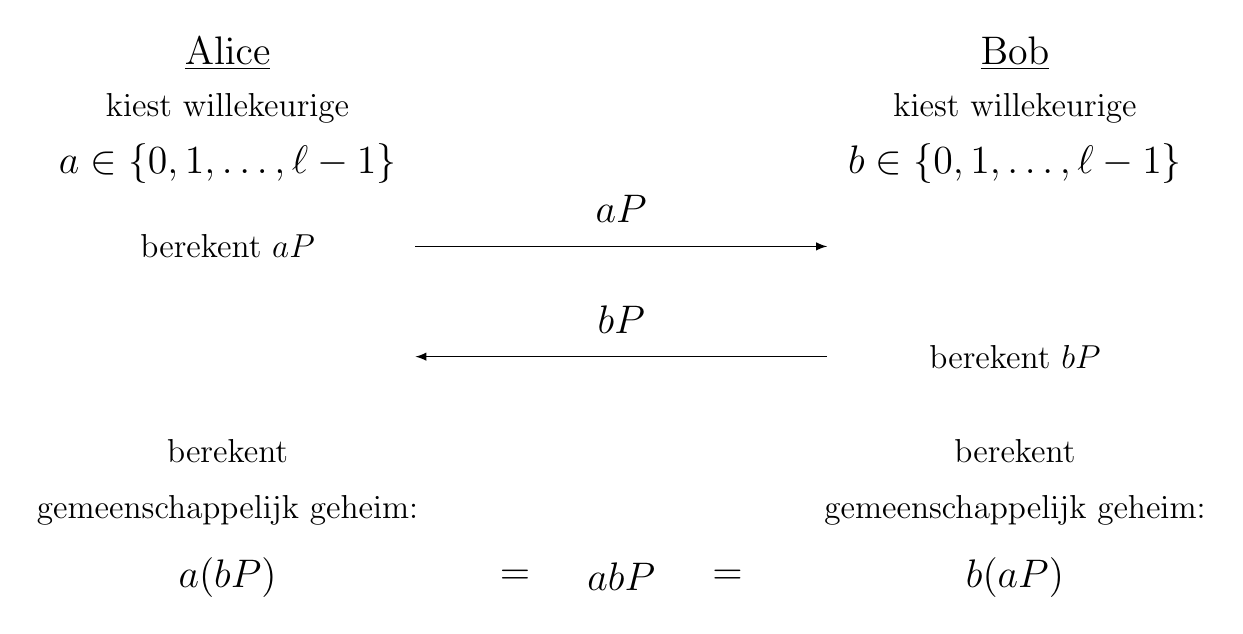
\begin{tikzpicture}[
    >=latex,
    textline/.style={
        font=\large,
        align=center
    },
    person/.style={
        font=\Large
    },
    formula/.style={
        font=\Large
    },
    message/.style={
        ->,
        thin,
        shorten >=1pt,
        shorten <=1pt
    }
]

% Horizontal positions of Alice and Bob
\def\AliceX{0}
\def\BobX{10}

% ==================================================
% Alice
% ==================================================

\node[person] at (\AliceX,4.8)
    {\underline{Alice}};

\node[textline] at (\AliceX,4.1)
    {kiest willekeurige};

\node[formula] at (\AliceX,3.4)
    {$a \in \{0,1,\ldots,\ell-1\}$};

\node[textline] at (\AliceX,2.35)
    {berekent $aP$};

% ==================================================
% Bob
% ==================================================

\node[person] at (\BobX,4.8)
    {\underline{Bob}};

\node[textline] at (\BobX,4.1)
    {kiest willekeurige};

\node[formula] at (\BobX,3.4)
    {$b \in \{0,1,\ldots,\ell-1\}$};

\node[textline] at (\BobX,0.95)
    {berekent $bP$};

% ==================================================
% Exchanged values
% ==================================================

% Alice sends aP to Bob
\draw[message]
    (2.35,2.35)
    --
    node[above=5pt, font=\Large] {$aP$}
    (7.65,2.35);

% Bob sends bP to Alice
\draw[message]
    (7.65,0.95)
    --
    node[above=5pt, font=\Large] {$bP$}
    (2.35,0.95);

% ==================================================
% Shared secret calculations
% ==================================================

% Alice's calculation
\node[textline] at (\AliceX,-0.25)
    {berekent};

\node[textline] at (\AliceX,-1.0)
    {gemeenschappelijk geheim:};

\node[formula] at (\AliceX,-1.85)
    {$a(bP)$};

% Bob's calculation
\node[textline] at (\BobX,-0.25)
    {berekent};

\node[textline] at (\BobX,-1.0)
    {gemeenschappelijk geheim:};

\node[formula] at (\BobX,-1.85)
    {$b(aP)$};

% Equality in the middle
\node[formula] at (3.65,-1.85) {$=$};
\node[formula] at (5.00,-1.85) {$abP$};
\node[formula] at (6.35,-1.85) {$=$};

\end{tikzpicture}